\documentclass[titlepage]{article}
\usepackage{graphicx} % Required for inserting images

\title{Informe Practica de Laboratorio 2}
\author{Cesar Rojas, \#31406902}
\date{Julio 2025}

\begin{document}

\maketitle

\section*{¿Qué diferencias existen entre registros temporales y registros guardados, cómo se aplicó esta distinción en la práctica?}

Los registros temporales (\emph{\$t0-\$t7}) no se preservan luego de una llamada a un procedimiento, mientras que los registros guardados (\emph{\$s0-\$s7}) se guardan en la pila (\emph{Stack}) al inicio de cada procedimiento que haga uso de ellos, y luego se restauran al finalizarse dicho procedimiento, preservándolos.

\section*{¿Qué diferencias existen entre los registros \emph{\$a0–\$a3, \$v0–\$v1, \$ra} y cómo se aplicó esta
distinción en la práctica?}

Los registros de argumento (\emph{\$a0-\$a3}) se usan para pasar parametros por argumento a un procedimiento antes de llamarlo, o para servir como argumentos de una llamada de sistema (\emph{syscall}).

Los registros de retorno (\emph{\$v0-\$v1}) se usan para retornar valores de procedimientos, y en el caso de \emph{\$v0} para determinar que tipo de llamada de sistema se va a realizar.

\emph{\$ra} se utiliza para guardar la dirección desde la cual se realizo la llamada de un procedimiento, para poder volver a esta una vez el procedimiento termine de ejecutarse.

\section*{¿Cómo afecta el uso de registros frente a memoria en el rendimiento de los algoritmos de ordenamiento implementados?}

Ya que los registros se encuentran directamente en el procesador en lugar de la RAM, estos son mucho mas rápido que cualquier memoria. Por lo tanto, usar registros en un algoritmo de ordenamiento resulta en una ejecución \emph{mucho} mas veloz, al poder acceder a los datos de forma inmediata en lugar de tener que extraerlos de la memoria.

\section*{¿Qué impacto tiene el uso de estructuras de control (\emph{bucles anidados, saltos}) en la eficiencia de los algoritmos en MIPS32?}

En el caso de los bucles anidado, cada uno introduce una nueva capa de iteraciones a ejecutar, aumentando secuencialmente el tiempo de ejecución según la complejidad de este, posiblemente en gran medida. Dependiendo de la complejidad del bucle base (asumamos $O(N)$), el primer bucle anidado la aumenta a $O(N^2)$, el segundo a $O(N^3)$, el tercero $O(N^4)$, y demás...

Los saltos son parte de las llamadas a procedimientos y lo que permiten que los bucles se repitan. Según su uso pueden o pueden no reducir la eficiencia del algoritmo, pero por si mismo no aumentan el orden de complejidad de un algoritmo.

\section*{¿Cuáles son las diferencias de complejidad computacional entre el algoritmo Bubble Sort y el algoritmo Selection Sort? ¿Qué implicaciones tiene esto para la implementación en un entorno MIPS32?}

El algoritmo Bubble Sort tiene una complejidad de $O(n)$ en el mejor caso, y de $O(n^2)$ en el peor, mientras que el algoritmo Selection Sort siempre es de complejidad $O(n^2)$.

En un entorno de MIPS32, esto resulta en que la implementación del algoritmo Selection Sort haga uso de mayor cantidad de registros, y esta recorre el vector una mayor cantidad de veces.

\section*{¿Cuáles son las fases del ciclo de ejecución de instrucciones en la arquitectura MIPS32 (camino de datos)? ¿En qué consisten?}

Las instrucciones en la arquitectura MIPS32 consisten, en general, de 5 fases: 
\begin{enumerate}
    \item \textbf{IF}: Consiste en obtener la instrucción de dentro de la memoria.
    \item \textbf{ID}: Decodifica dicha instrucción, y procede a leer los registros.
    \item \textbf{EX}: Utiliza el ALU para realizar la operación de la instrucción.
    \item \textbf{MEM}: Accede a la memoria de datos.
    \item \textbf{WB}: Y escribe dentro de esta el resultado.
\end{enumerate}

\section*{¿Qué tipo de instrucciones se usaron predominantemente en la práctica (\textbf{R, I, J}) y por qué?}

La mayoría de las funciones en la practica fueron de tipo \textbf{I}. Esto es debido a que estas forman la mayor parte de las instrucciones dentro de los bucles anidados, y estos son la parte del algoritmo que se ejecuta la mayor cantidad de veces.

Estas también se usan para transferir información entre registros (\emph{addi} y para realizar comparaciones (\emph{beq} y sus pseudo-instrucciones), ambas importantes para los algoritmos de ordenamiento.

\section*{¿Cómo se ve afectado el rendimiento si se abusa del uso de instrucciones de salto (\emph{j, beq, bne}) en lugar de usar estructuras lineales?}

Si no se usa una estructura lineal (arreglos, listas, pilas o colas) el numero de la instrucciones de salto aumenta exponencialmente, ya que cada cambio de posición haría falta de su propia iteración dentro de bucles anidados adicionales necesarios para recorrer la recorrer la memoria.

\section*{¿Qué ventajas ofrece el modelo RISC de MIPS en la implementación de algoritmos básicos como los de ordenamiento?}

Aunque el uso de un modelo RISC (\emph{Reduced Instruction Set Computer}) resulta en una mayor cantidad de código e instrucciones individuales, cada instrucción se ejecuta de forma mucho mas rapida ya que cada una es simple y especifica, lo que sirve para no solo compensar el aumento en instrucciones, si no para aumentar la eficiencia en general.

Esto es especialmente útil en algoritmos mas simples como los de ordenamiento, ya que estos no requieren de demasiado código MIPS para implementarse en comparación a algoritmos mas complejos.

\section*{¿Cómo se usó el modo de ejecución paso a paso (\emph{Step, Step Into}) en MARS para verificar la correcta ejecución del algoritmo?}

\begin{figure}[h]
    \centering
    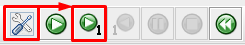
\includegraphics[width=0.75\textwidth]{images/step1.png} % 75% of text width
    \label{fig:step1}
\end{figure}

Primero, se compilo el archivo, y luego se recorrió paso a paso usando el botón '\emph{Run one step at a time}, remarcado en rojo. Cada paso ejecuta una instrucción, y con las siguientes ventanas se pudo observar los cambios que ocurrieron en cada uno.

\begin{figure}[h]
    \centering
    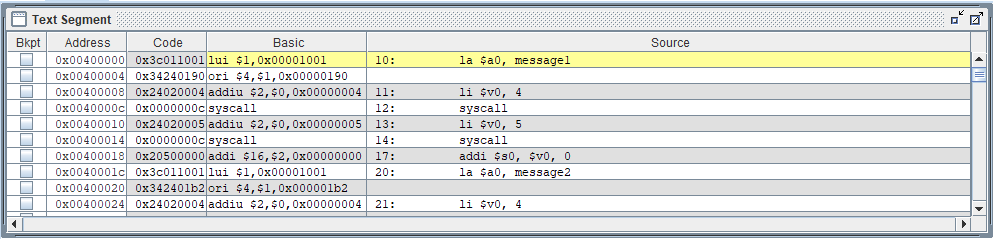
\includegraphics[width=0.75\textwidth]{images/step2.png} % 75% of text width
    \label{fig:step1}
\end{figure}

La ventana '\emph{Text Segment}' (segmento de texto) se utilizo para visualizar el recorrido, con el siguiente paso a ejecutar remarcado en amarillo.

\begin{figure}[h]
    \centering
    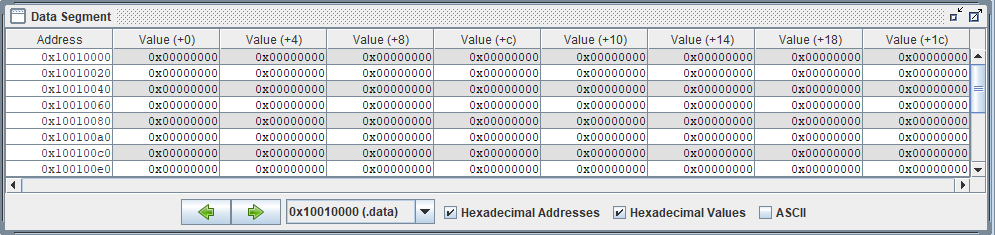
\includegraphics[width=0.75\textwidth]{images/step3.png} % 75% of text width
    \label{fig:step1}
\end{figure}

La ventana '\emph{Data Segment}' (segmento de datos) sirvió principalmente para visualizar el contenido de las estructuras lineales, como la pila y el vector que los algoritmos ordenaron.

\begin{figure}[h]
    \centering
    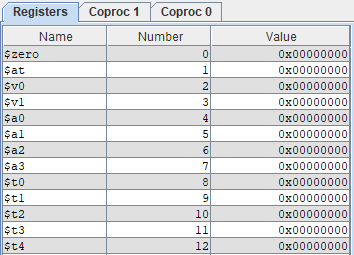
\includegraphics[width=0.75\textwidth]{images/step4.png} % 75% of text width
    \label{fig:step1}
\end{figure}

Finalmente, la ventana de registros fue la mas útil, sirviendo para poder observar el contenido de los registros mientras el algoritmo se ejecuto y observar cuando se cargaba información de manera incorrecta.

\section*{Justificar la elección del algoritmo alternativo}

Elegí el algoritmo Select Sort porque tiene una implementación similar a la del Bubble Sort, con dos bucles anidados que recorren el vector múltiples veces. A diferencia del Bubble Sort, Select Sort es menos eficiente ya que siempre tiene una complejidad de $O(N^2)$, a pesar de ser relativamente mas complicado.

En el Selection Sort también es necesario cambiar la posición de inicio del recorrido, en lugar de recorrer solo hasta N-i como Bubble Sort. La implementación de este tipo de recorrido opuesto parecía interesante, requiriendo el uso de un "apuntador" adicional que aumenta en cada recorrido.

\section{Análisis y Discusión de los Resultados}

Ambos algoritmos toman la misma entrada y retornan la misma salida final, e utilizan las mismas funciones para leer e imprimir vectores. Sin embargo, el método de ordenamiento difiere significativamente. Esto es observable al ejecutarlo paso a paso, en el segmento de datos, o al leer el resto de las salidas..

\begin{figure}[h]
    \centering
    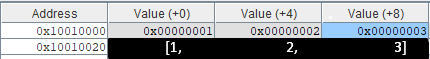
\includegraphics[width=0.75\textwidth]{images/step5.png} % 75% of text width
    \label{fig:step1}
\end{figure}

El elemento recién cambiado se marca en azul, y cada valor (+0, +4, +8...) corresponde a una posición del vector. Con esto es posible ver como este cambia durante la ejecución, y como el Selection Sort recorre el vector de forma distinta al Bubble Sort y como su ordenamiento es diferente.

La diferencia entre estos también es observable al simplemente ejecutar el programa. Se puede ver el estado del arreglo cada vez que se realiza un cambio, ya que este se imprime por pantalla.

\begin{itemize}
    \item El Bubble Sort recorre el algoritmo $N$ veces, mientras que el Selection Sort lo recorre $N^2$.
    \item El Selection Sort utiliza mas 'apuntadores' que Bubble Sort, en particular haciendo uso de un apuntador al inicio del vector que aumenta en 4 cada vez que se recorre (4, debido a la linealidad).
    \item Sus maneras de ordenar la lista son distintas. Selection Sort 'recuerda' cual es el elemento mas pequeño que encuentra en su recorrido y al final lo mueve a su posición correspondiente. Bubble Sort simplemente intercambia posiciones según las encuentra.
\end{itemize}

\end{document}
